\section{Methods}
\label{chapter:02}

% block-id: 02.conventions.heading
\hypertarget{02.conventions.heading}{}
\subsection{Operating conditions and comparison quantities}

% block-id: 02.conventions.p1
\hypertarget{02.conventions.p1}{}
Calculations use SI units, the exp(jωt) time convention, and RMS phasors. Copper at 20 °C has conductivity σ=5.8×10⁷ S/m and relative permeability μr=1. The principal transport condition is 200 kHz and 20 A RMS, with zero independent imposed field. Strands are insulated along their lengths and connected in parallel at their ends. Resistance and loss are normalized by axial length; actual strand arc lengths enter copper volume and DC resistance separately. Finite-segment terminal voltage is measured in V, while the two-dimensional axial terminal field is measured in V/m, with the chosen axial length connecting the two.

% block-id: 02.conventions.p2
\hypertarget{02.conventions.p2}{}
The original Q1 round wire, 2 mm in diameter, provides an analytical calibration. Its copper area is 3.141593 mm² and its mean DC current density at 20 A is 6.366198 A/mm², exceeding the specified limit of 4 A/mm². Q2 therefore requires at least 5 mm² copper cross-section. For 640 strands of copper diameter 0.100 mm, the ideal circular area is 5.026548 mm². Each strand in the two-dimensional model is represented by a 64-sided polygon, giving an actual copper area of \metric{coax_area} mm². Equal-copper comparisons use this discrete area so that the electromagnetic reference incorporates the same geometric approximation.

% block-id: 02.conventions.p3
\hypertarget{02.conventions.p3}{}
For unequal strand arc lengths, parallel conductances determine DC resistance and the sum of strand area–length products determines copper volume, as in \eqref{eq:E01}. We examine absolute AC resistance, Rac/Rdc, copper loss, and complex current sharing. Equation \eqref{eq:E02} gives RMS Joule loss and defines resistance from copper dissipation under pure transport excitation. The supplementary RT0 case uses an independent imposed field and zero net transport, so its absorbed power is reported separately as imposed-field loss.

% block-id: 02.equation.E01
\hypertarget{02.equation.E01}{}
\hypertarget{E01}{}
\begin{equation}
\begin{gathered}
R_{\mathrm{dc}}=\left(\sum_{k=1}^{N}\frac{\sigma A_k}{\ell_k}\right)^{-1} \\
V_{\mathrm{Cu}}=\sum_{k=1}^{N}A_k\ell_k
\end{gathered}
\tag{1}\label{eq:E01}
\end{equation}

% block-id: 02.equation.E02
\hypertarget{02.equation.E02}{}
\hypertarget{E02}{}
\begin{equation}
\begin{gathered}
P_{\mathrm{Cu}}=\int_{\Omega_{\mathrm{Cu}}}|\mathbf J|^2/\sigma\,\mathrm d\Omega \\
R_{\mathrm{ac}}=P_{\mathrm{Cu}}/|I_t|^2 \\
r_{\mathrm{ac}}=R_{\mathrm{ac}}/L_z
\end{gathered}
\tag{2}\label{eq:E02}
\end{equation}

% block-id: 02.hierarchy.heading
\hypertarget{02.hierarchy.heading}{}
\subsection{Model hierarchy and verification relationships}

% block-id: 02.hierarchy.p1
\hypertarget{02.hierarchy.p1}{}
The models are related as shown in Fig.~\ref{fig:model_hierarchy}. Analytical round-wire and two-dimensional diffusion models share the long, straight internal-field problem, allowing radial current and internal resistance to be compared. The two-dimensional common-terminal model additionally retains intrastand distributions, interstrand currents, and a controlled return, supporting field–circuit analysis of a specified cross-section. Longitudinal PEEC uses a finite-length partial-inductance kernel to examine the effect of length on axial currents. The three-component RT0 model uses imposed-field absorption in a cuboid to test three-dimensional continuity and discrete operators. Transposition paths and actual end regions require corresponding longitudinal or transverse degrees of freedom in subsequent structural research.

% block-id: 02.figure.model_hierarchy
\hypertarget{02.figure.model_hierarchy}{}
\begin{figure}[!htbp]
\centering
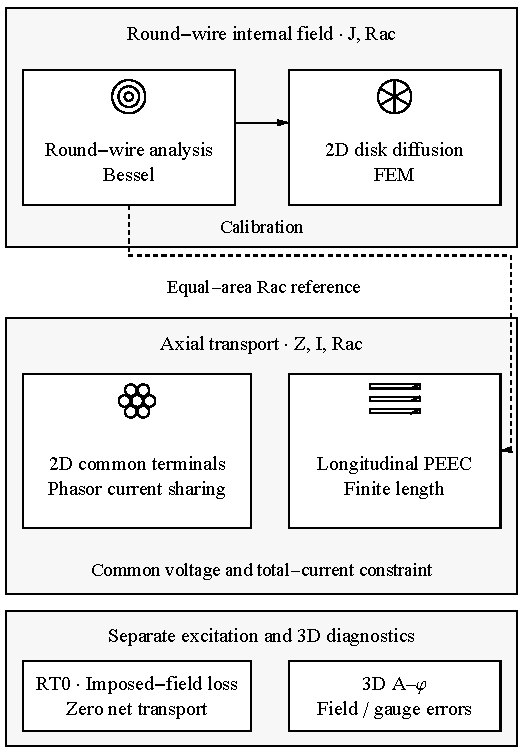
\includegraphics[width=\linewidth,height=.72\textheight,keepaspectratio]{../../assets/en/model_hierarchy.pdf}
\caption{Model hierarchy and comparable observables. Transport models are grouped by physical object and observable: round-wire internal fields support analytical and two-dimensional calibration, multistrand field–circuit models resolve common-terminal phasor currents, and longitudinal PEEC examines finite-length effects. Links identify internal-field calibration or equal-area resistance references. RT0 imposed-field loss and three-dimensional A–φ diagnostics occupy separate research scopes.}
\label{fig:model_hierarchy}
\end{figure}

% block-id: 02.hierarchy.p2
\hypertarget{02.hierarchy.p2}{}
Verification comprises equation solution, physical constraints, power consistency, and parameter sensitivity. Targets are 10⁻⁸ for true linear residuals, common-terminal conditions, and total complex current; 0.1\% for independent power balance; and 1\% for changes in mesh, segmentation, boundary, and length. Analytical reference values and current/power integrals use thresholds of 10⁻⁶ and 10⁻⁸, respectively. The RT0 GMRES true-residual target is 10⁻¹¹, its quadrature-sensitivity target is 0.1\%, and same-model CPU/GPU matrix and complex-current comparisons use 10⁻¹⁰.

% block-id: 02.hierarchy.p3
\hypertarget{02.hierarchy.p3}{}
These checks answer different questions. Residuals measure the accuracy of the discrete-system solution, power balance tests field–circuit and postprocessing consistency, and parameter sensitivity describes changes over specified perturbations. Model omissions, boundary approximations, and experimental deviations require their own evidence. We therefore distinguish numerical checks from physical applicability and interpret finite sensitivity studies as local validation rather than a common upper bound on total model error.

% block-id: 02.common.heading
\hypertarget{02.common.heading}{}
\subsection{Common-terminal coupling and uniform complex currents}

% block-id: 02.common.p1
\hypertarget{02.common.p1}{}
The common endpoints, strand branches, and return are related in Fig.~\ref{fig:common_terminal}. Let Z be the coupled impedance matrix of a specified linear model, e the independently induced voltage, i the complex strand currents, and V the common terminal voltage. The port equation Zi+e=V1 and total-current constraint 1\(^{\mathrm T}\)i=It form \eqref{eq:E04}. Solving the augmented system yields both magnitude and phase; It/N serves as a reference for the resulting current distribution.

% block-id: 02.equation.E04
\hypertarget{02.equation.E04}{}
\hypertarget{E04}{}\begin{equation}\begin{bmatrix} Z&-\mathbf1\\ \mathbf1^T&0\end{bmatrix}\begin{bmatrix}\mathbf i\\V\end{bmatrix}=\begin{bmatrix}-\mathbf e\\I_t\end{bmatrix}\tag{3}\label{eq:E04}\end{equation}

% block-id: 02.figure.common_terminal
\hypertarget{02.figure.common_terminal}{}
\begin{figure}[!htbp]
\centering
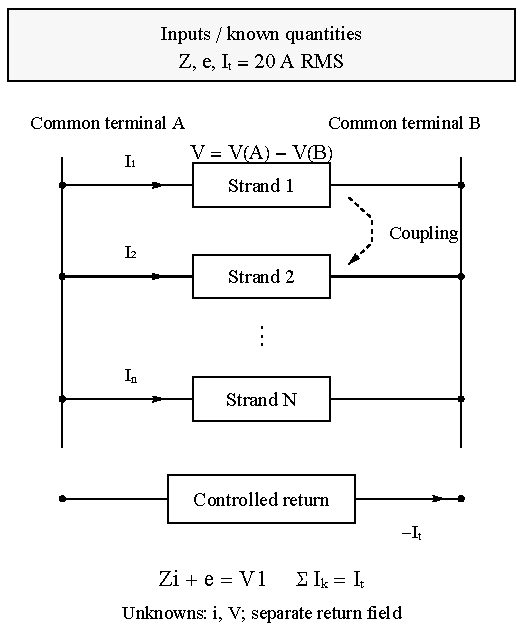
\includegraphics[width=\linewidth,height=.72\textheight,keepaspectratio]{../../assets/en/common_terminal.pdf}
\caption{Multistrand common terminals and return. Strands are insulated along their paths and connected in parallel at both ends; their phasor currents follow from the common voltage and total-current constraints. The coupling matrix Z and excitation term e contain the impedance and field contributions retained by the model. The controlled return carries the opposite total current and has its own terminal field. Known inputs and unknown currents and voltage are identified.}
\label{fig:common_terminal}
\end{figure}

% block-id: 02.common.p2
\hypertarget{02.common.p2}{}
When the augmented system has a unique solution, substitution of i=(It/N)1 shows that uniform currents exist if and only if every component of (It/N)Z1+e is equal. Projecting this vector onto the subspace orthogonal to 1 gives \eqref{eq:E05}. Without an independent imposed field, the condition reduces to equal row sums of Z; with an imposed field, the induced term also determines current sharing. This necessary and sufficient condition applies to the selected impedance model and terminal conditions, expressing the effect of transposition through changes in coupling and induced voltages.

% block-id: 02.equation.E05
\hypertarget{02.equation.E05}{}
\hypertarget{E05}{}
\begin{equation}
\begin{gathered}
Q=I_N-\mathbf1\mathbf1^T/N \\
Q\left[(I_t/N)Z\mathbf1+\mathbf e\right]=\mathbf0
\end{gathered}
\tag{4}\label{eq:E05}
\end{equation}

% block-id: 02.common.p3
\hypertarget{02.common.p3}{}
The two-dimensional common-terminal FEM solves the shared axial terminal field jointly with Az degrees of freedom. In conductors, Jz=σ(v−u), where both v and the saved variable u are expressed in V/m; the return conductor uses its corresponding terminal field. Current and loss are integrated on material-tagged linear triangles after coordinates are converted from mm to m. Strand currents, bundle loss, return loss, and copper area are independently compared with the original field–circuit results, treating air and conductor regions separately.

% block-id: 02.peec_method.heading
\hypertarget{02.peec_method.heading}{}
\subsection{Finite-length longitudinal PEEC}

% block-id: 02.peec_method.p1
\hypertarget{02.peec_method.p1}{}
Longitudinal PEEC divides the cross-section into volume filaments, each carrying an axial complex current density uniform along its length. Ohmic resistance and finite-volume partial inductance follow \eqref{eq:E08}, forming Z=R+jωL before the common-port and total-current constraints in \eqref{eq:E04} are applied. The counts 1264 and 5024 denote volume-filament degrees of freedom in a continuous conductor. Differences between their currents represent internal current concentration within the longitudinal basis.

% block-id: 02.equation.E08
\hypertarget{02.equation.E08}{}
\hypertarget{E08}{}
\begin{equation}
\begin{gathered}
R_{\alpha\beta}=\delta_{\alpha\beta}\frac{L_z}{\sigma A_\alpha} \\
L_{\alpha\beta}=\frac{\mu}{4\pi A_\alpha A_\beta}\int_{V_\alpha}\int_{V_\beta}\frac{\hat{\mathbf t}_\alpha\cdot\hat{\mathbf t}_\beta}{|\mathbf r-\mathbf r'|}\,\mathrm dV\,\mathrm dV'
\end{gathered}
\tag{5}\label{eq:E08}
\end{equation}

% block-id: 02.peec_method.p2
\hypertarget{02.peec_method.p2}{}
The longitudinal case has a nominal round-wire diameter of 2 mm. The m40 and m80 square filaments are 0.050 and 0.025 mm wide, giving actual cross-sectional areas of 3.16 and 3.14 mm². Sensitivity studies vary length, mutual integration, or self integration independently. The 1264-degree-of-freedom model uses one cross-section at lengths 0.16, 0.32, and 0.64 m. At fixed length, mutual quadrature order q is increased through 4, 6, and 8, while self-integration settings increase from 10/8 to 12/10. These pairs are AccuracyGoal and PrecisionGoal, the target absolute and relative precision digits. The 5024-degree-of-freedom model checks lengths 0.32 and 0.64 m and the same integration changes. Because the two cross-sectional discretizations have slightly different copper areas, each resistance is compared with its own equal-area Bessel reference; changes between discretizations include both discretization and area approximation.

% block-id: 02.peec_method.p3
\hypertarget{02.peec_method.p3}{}
The partial-inductance kernel includes magnetic coupling around finite conductors, whereas the Bessel solution gives the internal impedance of a long straight round wire. We compare their dissipative component Rac while retaining length and area conditions. The length study measures sensitivity of the current kernel and longitudinal basis. Transverse loops, curved strands, and actual end-current redistribution require extended degrees of freedom. The connection to FEM–PEEC coupling \cite{P03} lies in a joint field–circuit description; excitation, return, and field-feedback choices must be compared for each implementation.
